All considered metrics are defined by terms from the so-called confusion matrix shown in Figure~\ref{fig:2_basics/4_metrics/1_confusion_matrix}. The matrix applies to the general scenario in which predictions are made about a certain condition for a set of objects. Thereby, an object's actual condition can be positive or negative, also referred to as its \emph{ground truth}, as can be the object's predicted condition. A prediction is \emph{true}, or correct, if its predicted condition is consistent with the object's actual condition and \emph{false} otherwise. Furthermore, objects whose prediction is positive are called \emph{positives}, while objects whose predictions are negative are called \emph{negatives}. Depending on their actual and their predicted condition, each object falls into one of four distinct categories:

\begin{figure}[t]
    \centering
    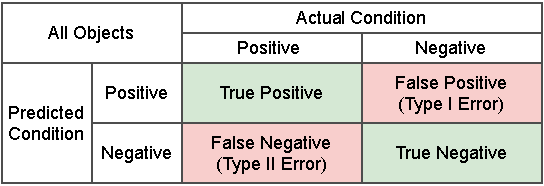
\includegraphics[width=\textwidth]{2_basics/4_metrics/1_confusion_matrix/confusion_matrix}
    \caption{Confusion Matrix dividing objects into four distinctive groups depending on their actual and predicted condition}
    \label{fig:2_basics/4_metrics/1_confusion_matrix}
\end{figure}

\begin{itemize}
    \item \textbf{\emph{True positives}} (TP) are objects for which the regarded condition is positive and whose predicted conditions is also positive.

    \item \textbf{\emph{False positives}} (FP) are objects for which the regarded condition is positive but whose predicted condition is negative. This type of error is referred to as a \emph{Type I error}.

    \item \textbf{\emph{False negatives}} (FN) are objects for which the condition is actually negative but whose predicted condition is positive. This second kind of errornous prediction is also referred to as \emph{Type II error}.

    \item \textbf{\emph{True negatives}} (TN) are objects for which the condition is actually negative and whose predicted condition is also negative.
\end{itemize}

Although it is generally desirable to obtain as many correct predictions as possible, true positives and true negatives are often differently important and errors of type one and two differently severe. In medicine, for example, not recognizing a disease could be much worse than accidentally diagnosing a healthy person as ill. Conversely, not recognizing guilt in a lawsuit might be less serious than convicting someone who is innocent. In the context of knowledge graph completion under the open-world assumption, the focus lies on true positives since the KGC model cannot make any qualified statements about false facts without negative samples in the graph. Omitting a fact from the prediction only means that the model has too little evidence for that fact, not that it can falsify it.
